\documentclass{article}
\usepackage[utf8]{inputenc}
\usepackage[top=1in]{geometry}
\usepackage{graphicx}
\usepackage{booktabs}
\usepackage{amsmath}
\usepackage{amsthm}
\usepackage[only]{excludeonly}
\usepackage{fancyhdr}
\usepackage{tikz}
\usetikzlibrary{circuits.logic.US,positioning,calc} 
\usepackage[american]{circuitikz}

\usepackage{enumitem,amssymb}
\newlist{todolist}{itemize}{2}
\setlist[todolist]{label=$\square$}
\usepackage{pifont}
\newcommand{\cmark}{\ding{51}}%
\newcommand{\xmark}{\ding{55}}%
\newcommand{\done}{\rlap{$\square$}{\raisebox{2pt}{\large\hspace{1pt}\cmark}}%
  \hspace{-2.5pt}}
\newcommand{\wontfix}{\rlap{$\square$}{\large\hspace{1pt}\xmark}}

\input{karnaugh}
\input{sym}
\title{ECE275 Midterm 1 Fall 2022}
\author{Instructor: Vikas Dhiman (\texttt{vikas.dhiman@maine.edu})}
\newtheorem{example}{Example}
\newtheorem{prob}{Problem}
\newtheorem{remark}{Remark}

\newcommand{\bx}{\bar{x}}
\newcommand{\by}{\bar{y}}
\newcommand{\bz}{\bar{z}}
\newcommand{\bX}{\bar{X}}
\newcommand{\bY}{\bar{Y}}
\newcommand{\bZ}{\bar{Z}}
\newcommand{\bA}{\bar{A}}
\newcommand{\bB}{\bar{B}}
\newcommand{\bC}{\bar{C}}

\fancyhead[LH]{Name: \hspace{10em}}
\fancyhead[RH]{Email: \hspace{10em}}
\includeonly{0930-sample-exam}
\begin{document}


\section{Syllabus covered}

\begin{itemize}
  \item[\done] Binary numbers
  \item[\done] Generate minterms, maxterms, SOP canonical form and POS
    canonical forms and convert between them\\
  \item[\done]  Understand and use the laws and theorems of Boolean Algebra
  \item[\done]  Perform algebraic simplification using Boolean algebra
  \item[\done]  Simplification using K-maps
  \item[\done]  Derive sum of product and product of sums expressions for a combinational circuit
  \item[\done]  Convert combinational logic to NAND-NAND and NOR-NOR forms
  %\item[\done]  Simplification using Quine-McCluskey method, PI tables and Petrick's method
  \item Hexadecimal, Sign-magnitude, One's-complement and
    Two's complement. Conversions between them.
  \item  Design combinational circuits for positive and negative logic
  \item  Design Hazard-free two level circuits and understand Hazards in multi-level circuits
  \item Compute noise margin of one device
  \item Describe how tri-state and open-collector outputs are different from totem-pole outputs.
  \item Different between and limitations of master-slave and edge-triggered flip-flops.
  \item Compute fan out and noise margin of one device driving the same time
  \item Know the differences and similarities between PAL, PLA, and ROMs and can use each for logic design
  \item Design combinational circuits using multiplexers and decoders
  \item Analyze a sequential circuit and derive a state-table and a state-graph
  \item Understand the difference between synchronous and asynchronous inputs
  \item Derive a state graph or state table from a word description of the problem
  \item Reduce the number of states in a state table using row reduction and implication tables
  \item Perform a state assignment using the guideline method
  \item Implement a design using JK, SR, D or T flip-flops
  \item Analyse and design both Mealy and Moore sequential circuits with multiple inputs and multiple outputs
  \item Convert between Mealy and Moore designs
  \item Partition a system into multiple state machines
\end{itemize}

\subsection{Labs (not questioned in exams)}
\begin{itemize}
  \item Use computer tools to enter designs graphically and HDL
  \item Simulate designs using computer tools
  \item Use computer tools to program gate arrays logic and debug and test
\end{itemize}

\newpage


\maketitle

Student Name: \hfill Student Email: \hspace{10em}
\section{Instructions}
\begin{itemize}
  \item Time allowed is 50 minutes. (This sample exam might be lengthier than the actual exam. )
  \item In order to minimize distraction to your fellow students, you may not leave
  during the last 10 minutes of the examination.
  \item The examination is closed-book. One 8x11in cheatsheet is allowed.
  \item Non-programmable calculators are permitted.
  \item The maximum number of marks is 100, as indicated; the midterm examination
  amounts 10\% toward the final grade.
  \item Please use a pen or heavy pencil to ensure legibility.
  \item Please answer questions in the spaces provided; if space is insufficient, please
  use the back of the pages.
  \item Please show your work; where appropriate, marks will be awarded for proper and well-reasoned explanations.
\end{itemize}

\begin{prob}
  Number conversions:
  \begin{enumerate}
    \item Use repeated division to convert $230_{10}$ to octal representation (5 marks).
    \item What is the value of $19D_{16}$ in base 10 (5 marks).
    \item A 6-bit two's complement number is $100011_{2}$. Convert it to (signed) decimal (5 marks).
    \item Represent $-23_{10}$ in two's complement binary notation (5 marks).
  \end{enumerate}
\end{prob}

\begin{prob}
  Consider the circuit below\\
  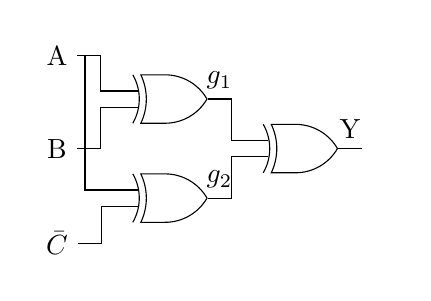
\begin{tikzpicture}[circuit logic US]
    \matrix[column sep=7mm]
    {
      \node (A) {A}; &  &  & \\
      & \node [xor gate] (AxorB) {}; &  &\\
      \node (B) {B}; &  & \node [xor gate] (f) {}; \\
      & \node [xor gate] (BxorC) {}; &  & \\
      \node (C) {$\bC$}; &  & &\\
    };
    \draw (A.east) --++(right:3mm) |- (AxorB.input 1);
    \draw (B.east) --++(right:3mm) |- (AxorB.input 2);
    \draw (A.east) --++(right:1mm) |- (BxorC.input 1);
    \draw (C.east) --++(right:3mm) |- (BxorC.input 2);
    \draw (AxorB.output) to [edge label=$g_1$] ++(right:3mm) |- (f.input 1);
    \draw (BxorC.output) to [edge label=$g_2$] ++(right:3mm) |- (f.input 2);
    \draw (f.output) to [edge label=Y] ++(right:3mm) ;
  \end{tikzpicture} \\
  By algebraic manipulation, prove or disprove that $Y = \bB \bC + B C$ (10 marks).
\end{prob}

\begin{prob}
Use the following 5-variable K-map for F (A, B, C, D, E), and find
  a minimal SOP expression for F (15 marks)\\
\begin{minipage}{0.5\linewidth}
  \centering
  \begin{Karnaugh}{BC}{DE}
    \minterms{0,1,5,6,7,8,9,14}
  \end{Karnaugh}\\
  A=0
\end{minipage}%
\begin{minipage}{0.5\linewidth}
  \centering
  \begin{Karnaugh}{BC}{DE}
    \minterms{1,4,5,6,7,9,12,14}
  \end{Karnaugh}\\
  A=1
\end{minipage}
\end{prob}

\begin{prob}
  Use bubble-pushing and/or algebra to find an SOP expression
for Y in the circuit below. If you use bubble-pushing, draw an equivalent
  circuit beside the given circuit (5 marks).\\
  \includegraphics[width=0.4\linewidth]{figures/bubble-pushing-circuit.png}
\end{prob}

\begin{prob}
  Consider the function Y given below.
  \[ Y(A, B, C, D) = \sum m(0, 3, 5, 7, 8, 14) + d(2, 12, 15) \]
  \begin{enumerate}
    \item Draw a K-maps to derive a minimum SOP and POS expressions for Y .
      Indicate all essential prime implicants for Y or $\bY$ in your K-maps (20 marks).
    \item Sketch a two-level NOR-NOR circuit for Y. Assume that A, B, C, and D are available in true end complimentary forms (5 marks).
    \item Write Y in Product of sums (POS) \emph{canonical} form (5 marks).
  \end{enumerate}
\end{prob}

\begin{prob}
  Design a minimal SOP circuit to add two two-bit unsigned numbers. Denote the two bits of first number as $A_1A_0$ and the two bits of second number as $B_1B_0$. The result will be a 2-bit sum $S_1S_0$ and a carry $C$. Start with filling out the following truth table (3 example rows are provided) and then use K-maps to find minimal SOP for $S_1$, $S_0$ and a single carry bit $C_1$ (20 marks).
  \begin{tabular}{cccc|ccc}
    \toprule
    $A_1$ & $A_0$ & $B_1$ & $B_0$ & $C_1$ & $S_1$ & $S_0$  \\
    \midrule
    0 & 0 & 0 & 0 &   &   &   \\
    0 & 0 & 0 & 1 &   &   &   \\
    0 & 0 & 1 & 0 &   &   &   \\
    0 & 0 & 1 & 1 &   &   &   \\
    0 & 1 & 0 & 0 &   &   &   \\
    0 & 1 & 0 & 1 & 0 & 1 & 0 \\
    0 & 1 & 1 & 0 &   &   &   \\
    0 & 1 & 1 & 1 &   &   &   \\
    1 & 0 & 0 & 0 &   &   &   \\
    1 & 0 & 0 & 1 &   &   &   \\
    1 & 0 & 1 & 0 &   &   &   \\
    1 & 0 & 1 & 1 &   &   &   \\
    1 & 1 & 0 & 0 &   &   &   \\
    1 & 1 & 0 & 1 & 1 & 0 & 0 \\
    1 & 1 & 1 & 0 &   &   &   \\
    1 & 1 & 1 & 1 & 1 & 1 & 0 \\
    \bottomrule
  \end{tabular}
\end{prob}


%\bibliography{main}
%\bibliographystyle{plain}
\end{document}
